\chapter{SIIT-DCのデザインと現状の課題}
\label{issue}
第\ref{related:compare:translation}で述べたPv4/IPv6トランスレーションを用いたIPv4サービス提供手法の一つとして,SIIT-DCがインターネット標準化されている.
本章ではてSIIT-DCのデザインとメリット及び考えられる運用,そして現状の課題について述べる.
\section{SIIT-DC}
\label{issue:siit-dc}


\subsection{概要}
SIIT-DCとは,ステートレスIP/ICMP変換アルゴリズム\cite{RFC7915}を利用して,IPv4インターネット・ネットワークからのアクセスをIPv6シングルスタックネットワーク上のホストに提供するためのネットワークデザインである.2016年よりIETF IPv6 Operations WG\footnote{IPv6ネットワークの運用要件や関連する技術仕様の策定を行うワーキンググループ.\url{https://datatracker.ietf.org/wg/v6ops/about/}}によりインターネット標準化(Informational RFC)されている\cite{RFC7755}.


\subsection{用語}
\label{issue:siit-dc:terms}
SIIT-DCで利用される用語及び特殊な役割を有する機器・技術について述べる.

\subsubsection{SIIT}
SIIT\footnote{Stateless IP/ICMP Translation Algorithm}とはIPv4/IPv6トランスレーションに用いられるプロトコル変換機能の略称である.RFC2765\cite{RFC2765}で初めて標準化され,その後RFC6145\cite{RFC6145}により一部の仕様が実運用のユースケースに合わせて変更され,現在はIPv6拡張ヘッダーを扱う機構などが追加されたRFC7915\cite{RFC7915}が現行の標準仕様である.

\subsubsection{BR}
BR\footnote{Border Relay}とは,SIIT-DCネットワークにおいてIPv4インターネットとIPv6ネットワークとの間でSIITによるIPv4/IPv6トランスレーションを行う機器\footnote{専用機器もしくは他の役割を有する機器の一機構.}である.
IPv4インターネットとIDC内のIPv6シングルスタックネットワークの各境界部に所在し,後述するEAMTを参照した1:1のアドレス変換を行う.IDCネットワークにIPv4インターネットとの接続点が複数ある場合,接続点ごとに最低一つのBRを配備する.

\subsubsection{ER}
ER\footnote{Edge Relay}とは,IPv4ネットワークとIPv6ネットワークとの境界点において多:多のIPv4/IPv6トランスレーションを行う機器である.
SIIT-DCではそのオプションとして,IPv4ネットワーク内のIPv4しか利用出来ないホストが,SIIT-DCを利用してIPv4サービスを提供するユースケースをサポートするSIIT-DC Dual Translation Mode\cite{RFC7756}が定義されており,ERはその中での利用が想定されている.

通常,ERが参照するEAMT中のEAMはIDCネットワーク内のIPv4ネットワーク全体を包括的に指定したIPv4ネットワークアドレスと,そのIPv4ネットワークを表すIPv6サービスアドレスにより構成される.

\subsubsection{IPv4サービスアドレス}
IPv4サービスを提供するIPv6シングルスタックネットワークに属するホストに割り当てるIPv4アドレス(群)をIPv4サービスアドレスと呼称する.
このアドレス宛に送信されたパケットは,BR/ERによって対応するIPv6サービスアドレスに変換される.

なお,IPv4サービスアドレスはBGP\cite{RFC4271}によってIPv4インターネットに経路広告されている必要がある.

\subsubsection{IPv6サービスアドレス}
ER/BRを介してアプリケーションやホストに割り当てられたIPv6アドレス(群)をIPv4サービスアドレスと呼称する.
IPv4クライアントはSIIT-DCのアーキテクチャをを介して,このIPv6サービスアドレスが割り当てられたホストと通信することが出来る.

\subsubsection{変換プレフィックス}
\label{issue:siit-dc:translation-prefix}
 
変換プレフィックス\footnote{Translation Prefix.}とは,RFC6052\cite{RFC6052}で定義されたプロトコルに従って全てのIPv4アドレスをマッピングするために用いられるネットワークプレフィックスが96bitのIPv6プレフィックスである.IANAによって主にWKP\footnote{Well Known Prefix. }として64:ff9b::/48が予約\cite{RFC8215,IANA_allocation_v6}されているが,運用者の裁量でISP自身に割り当てられたNSP\footnote{Network Specific Prefx. 主にRIRから割り当てられたIPv6 Global Unicas Addressを指す.}を利用する事ができる.

IPv4アドレスとIPv6アドレスの間で変換を実行する際に,BはBR/ERは変換前のIPヘッダーのアドレスフィールドを、変換プレフィックスが挿入・削除された状態に書き換える。

なおSIIT-DCネットワークにおいて,変換プレフィックス宛のパケットは各BR/ERのIPv6インターフェース宛にIGP\footnote{Interior Gateway Protocol}などでルーティングされる必要がある.

\subsubsection{EAM}
EAM\footnote{Ecplicit Address Mapping}とは,EAMアルゴリズム\cite{RFC7757}によって結びつけられたIPv4サービスアドレスとIPv6サービスアドレスのペア\footnote{サービスアドレスはそれぞれネットワークプレフィックスとして指定することも想定されている.}を表す.

EAMにおいて,IPv4サービスアドレスとIPv6サービスアドレスは同数\footnote{標準では結び付けられたIPv6サービスアドレスがIPv4サービスアドレスより多い状態が想定されているが,IPv6サービスアドレスのホスト部が若いものから優先して変換するため,余剰分のアドレスは無視される.}である必要がある.

また,BR及びERが変換を行う際に参照するEAM群が記録されたテーブルをEAMT\footnote{Ecplicit Address Mapping}と定義している.以後EAMTもしくは変換テーブルと呼称する.



\subsection{ネットワーク設計}
\label{issue:siit-dc:network}
\begin{figure}[h]
    \begin{center}
      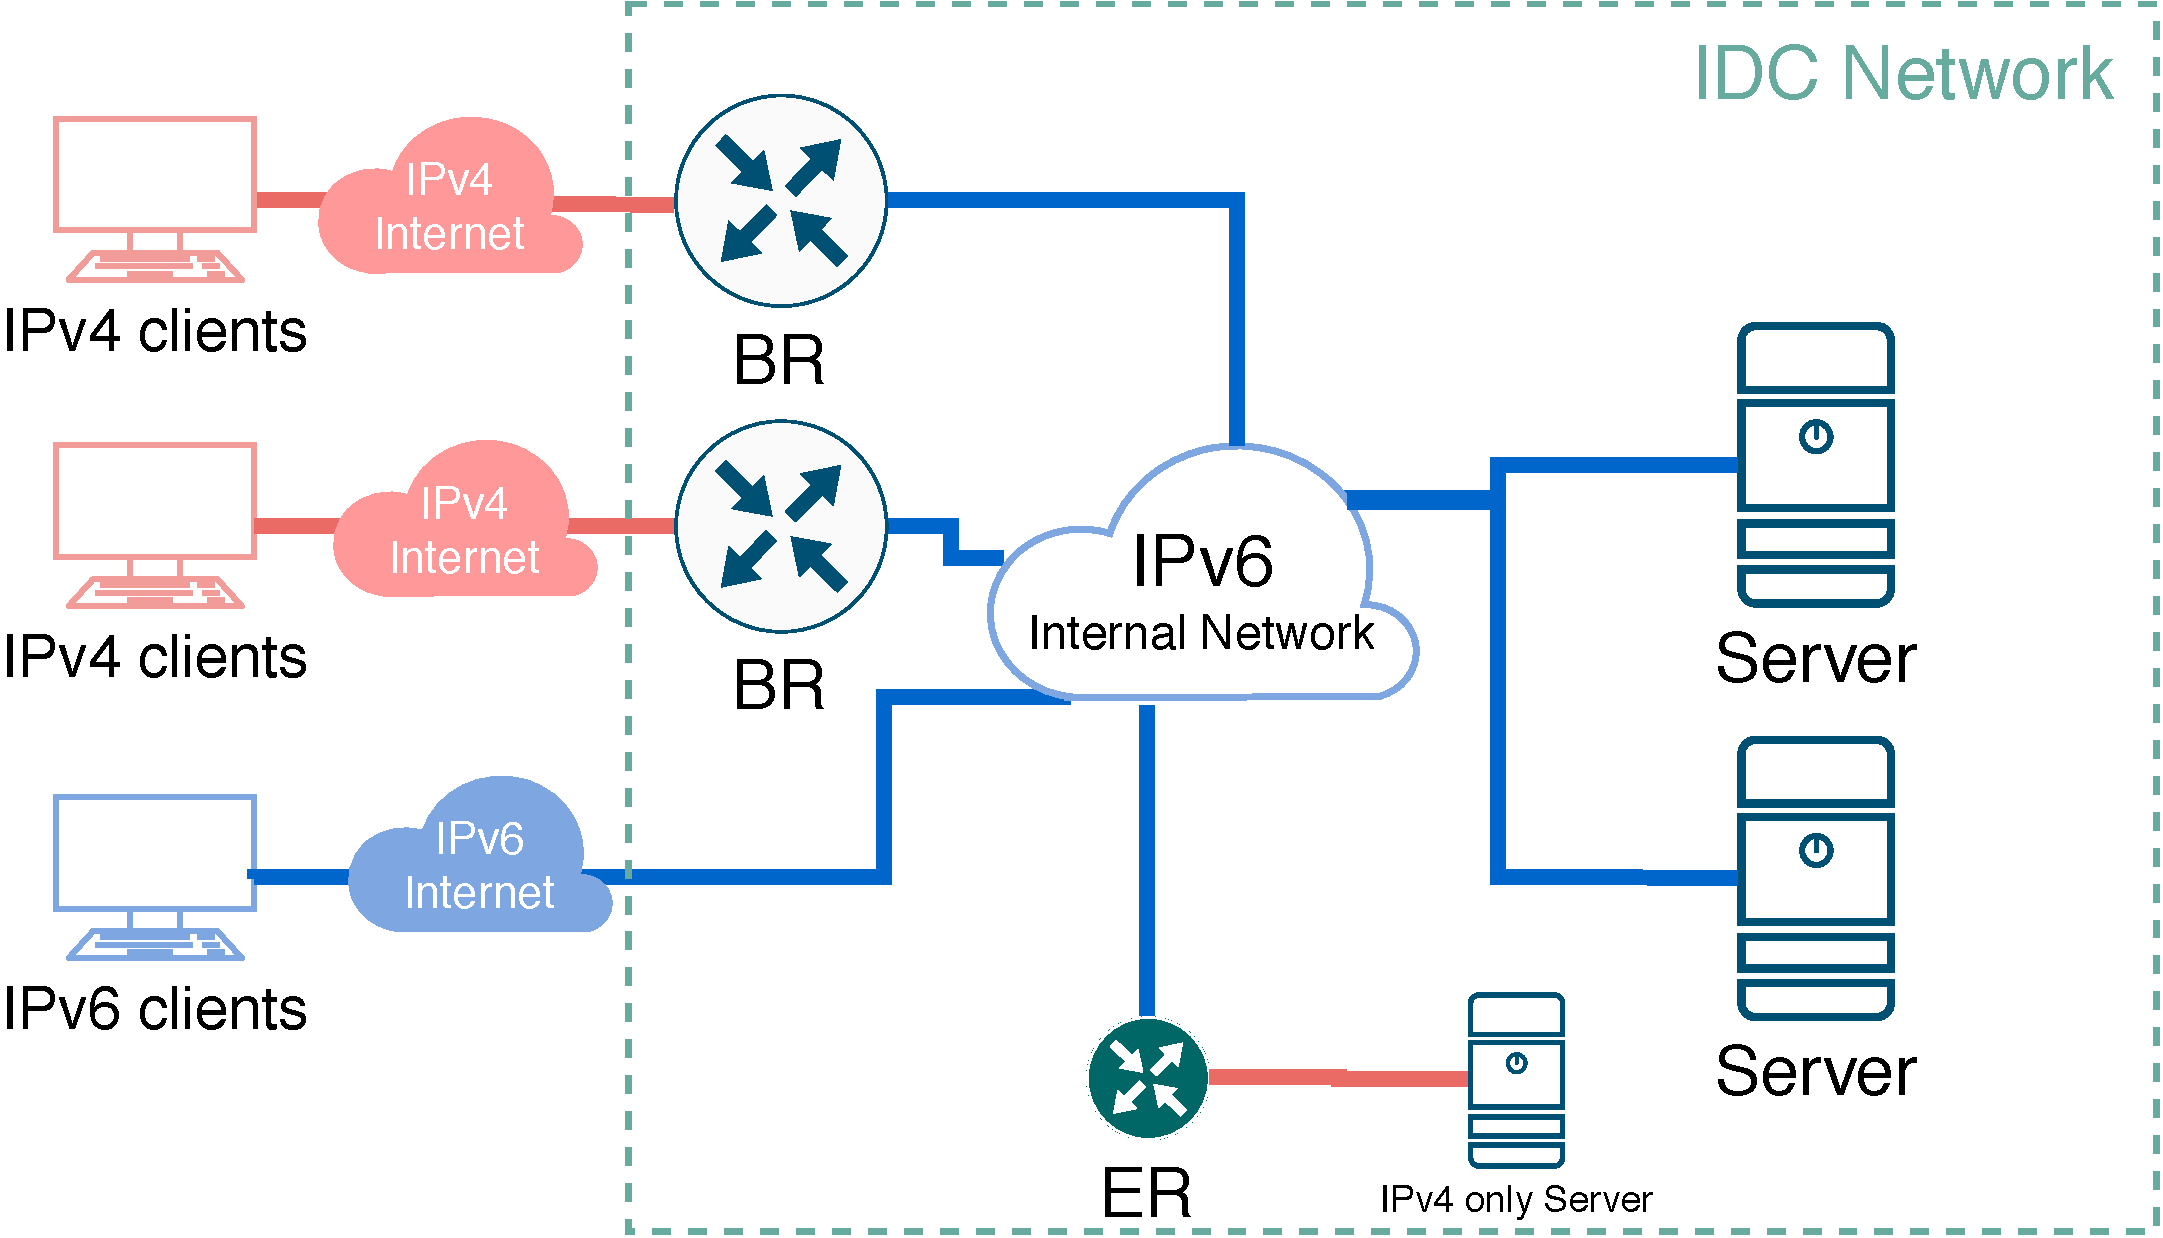
\includegraphics[width=12cm,pagebox=cropbox,clip]{img/siit-dc-network.pdf}
    \end{center}
    \caption{SIIT-DC ネットワーク}
    \label{fig:siit-dc_network}
\end{figure}
基本的なSIIT-DCネットワークを図\ref{fig:siit-dc_network}に示す.

BRはIPv4インターネットとの各接続点に配置される.各IPv4サービスアドレスはBGPにより接続先のAS\footnote{Aunotoumous System. インターネットを構成する自律した組織.}に対して経路広告される.変換プレフィックス宛のパケットは各BRに広告される.

BRが複数ある場合,それぞれのBRがIGP等で広告する変換プレフィックスを分けるか,エニーキャスト\cite{RFC4786}によって複数のBRが同一の変換プレフィックスを広告するようにする.エニーキャストを使用した場合,BRの障害時に別のBRへとトラフィックを迂回させることが可能になる.

ERはIDC内のIPv4ネットワークとの接続点に配置され,IPv4のみを持つホストがIDC内のIPv6ネットワークを介してIPv4インターネットにサービス提供を行う場合に利用される.


\subsection{SII-DCのメリット}
\label{issue:siit-dc-merit}
SIIT-DCを用いたIPv4サービスの提供によるメリットとして,以下の様な物が挙げられる,

\subsubsection{デプロイメントが容易}
SIIT-DCは,IDCのIPv6ネットワークとIPv4インターネットとの接続点にBRを設置を行うのみで,対外的な基本的なIPv4サービスの提供が可能だ.
そのためIDCのネットワークトポロジーに限定されないシンプルなIPv4サービス提供が期待できる.

\subsubsection{アドレス単位でのIPv4アドレスの効率的な利用が可能}
通常のIPネットワークでは,サブネット単位での割当が必要である.従来,事前に同一サブネットに属するホスト数を見積持った上で不足が生じないようになネットワークサイズを設定しする必要があっため,ネットワークサイズをを超えるサービスの拡大が必要になった場合,サブネット全体の再設計が不可欠であった.またIPネットワークには,ネットワークアドレスやブロードキャストアドレス,そしてデフォルトゲートウェイとなるルーターのインターフェースのアドレスを確保する必要があり,ネットワークサイズが断片化されるほど,実質的に利用できないアドレスの割合が大きくなる問題が会った.

しかしながらSIIT-DCではアドレス単位でのIPv4提供サーバーへの割当が可能である.すなわち,従来利用できなかったIPv4アドレスを再利用することで,IPv4アドレスの効率的な活用を実現できる.第\ref{introduction:background:ipv4_problems}で述べたように今後益々IPv4アドレスの調達が難しくなっているため,IPv4アドレスの効率的な利用は事業者の負担軽減に繋がる.

\subsubsection{スケーラビリティ}
\label{issue:siit-dc-merit:scalability}
\begin{figure}[h]
  \begin{center}
    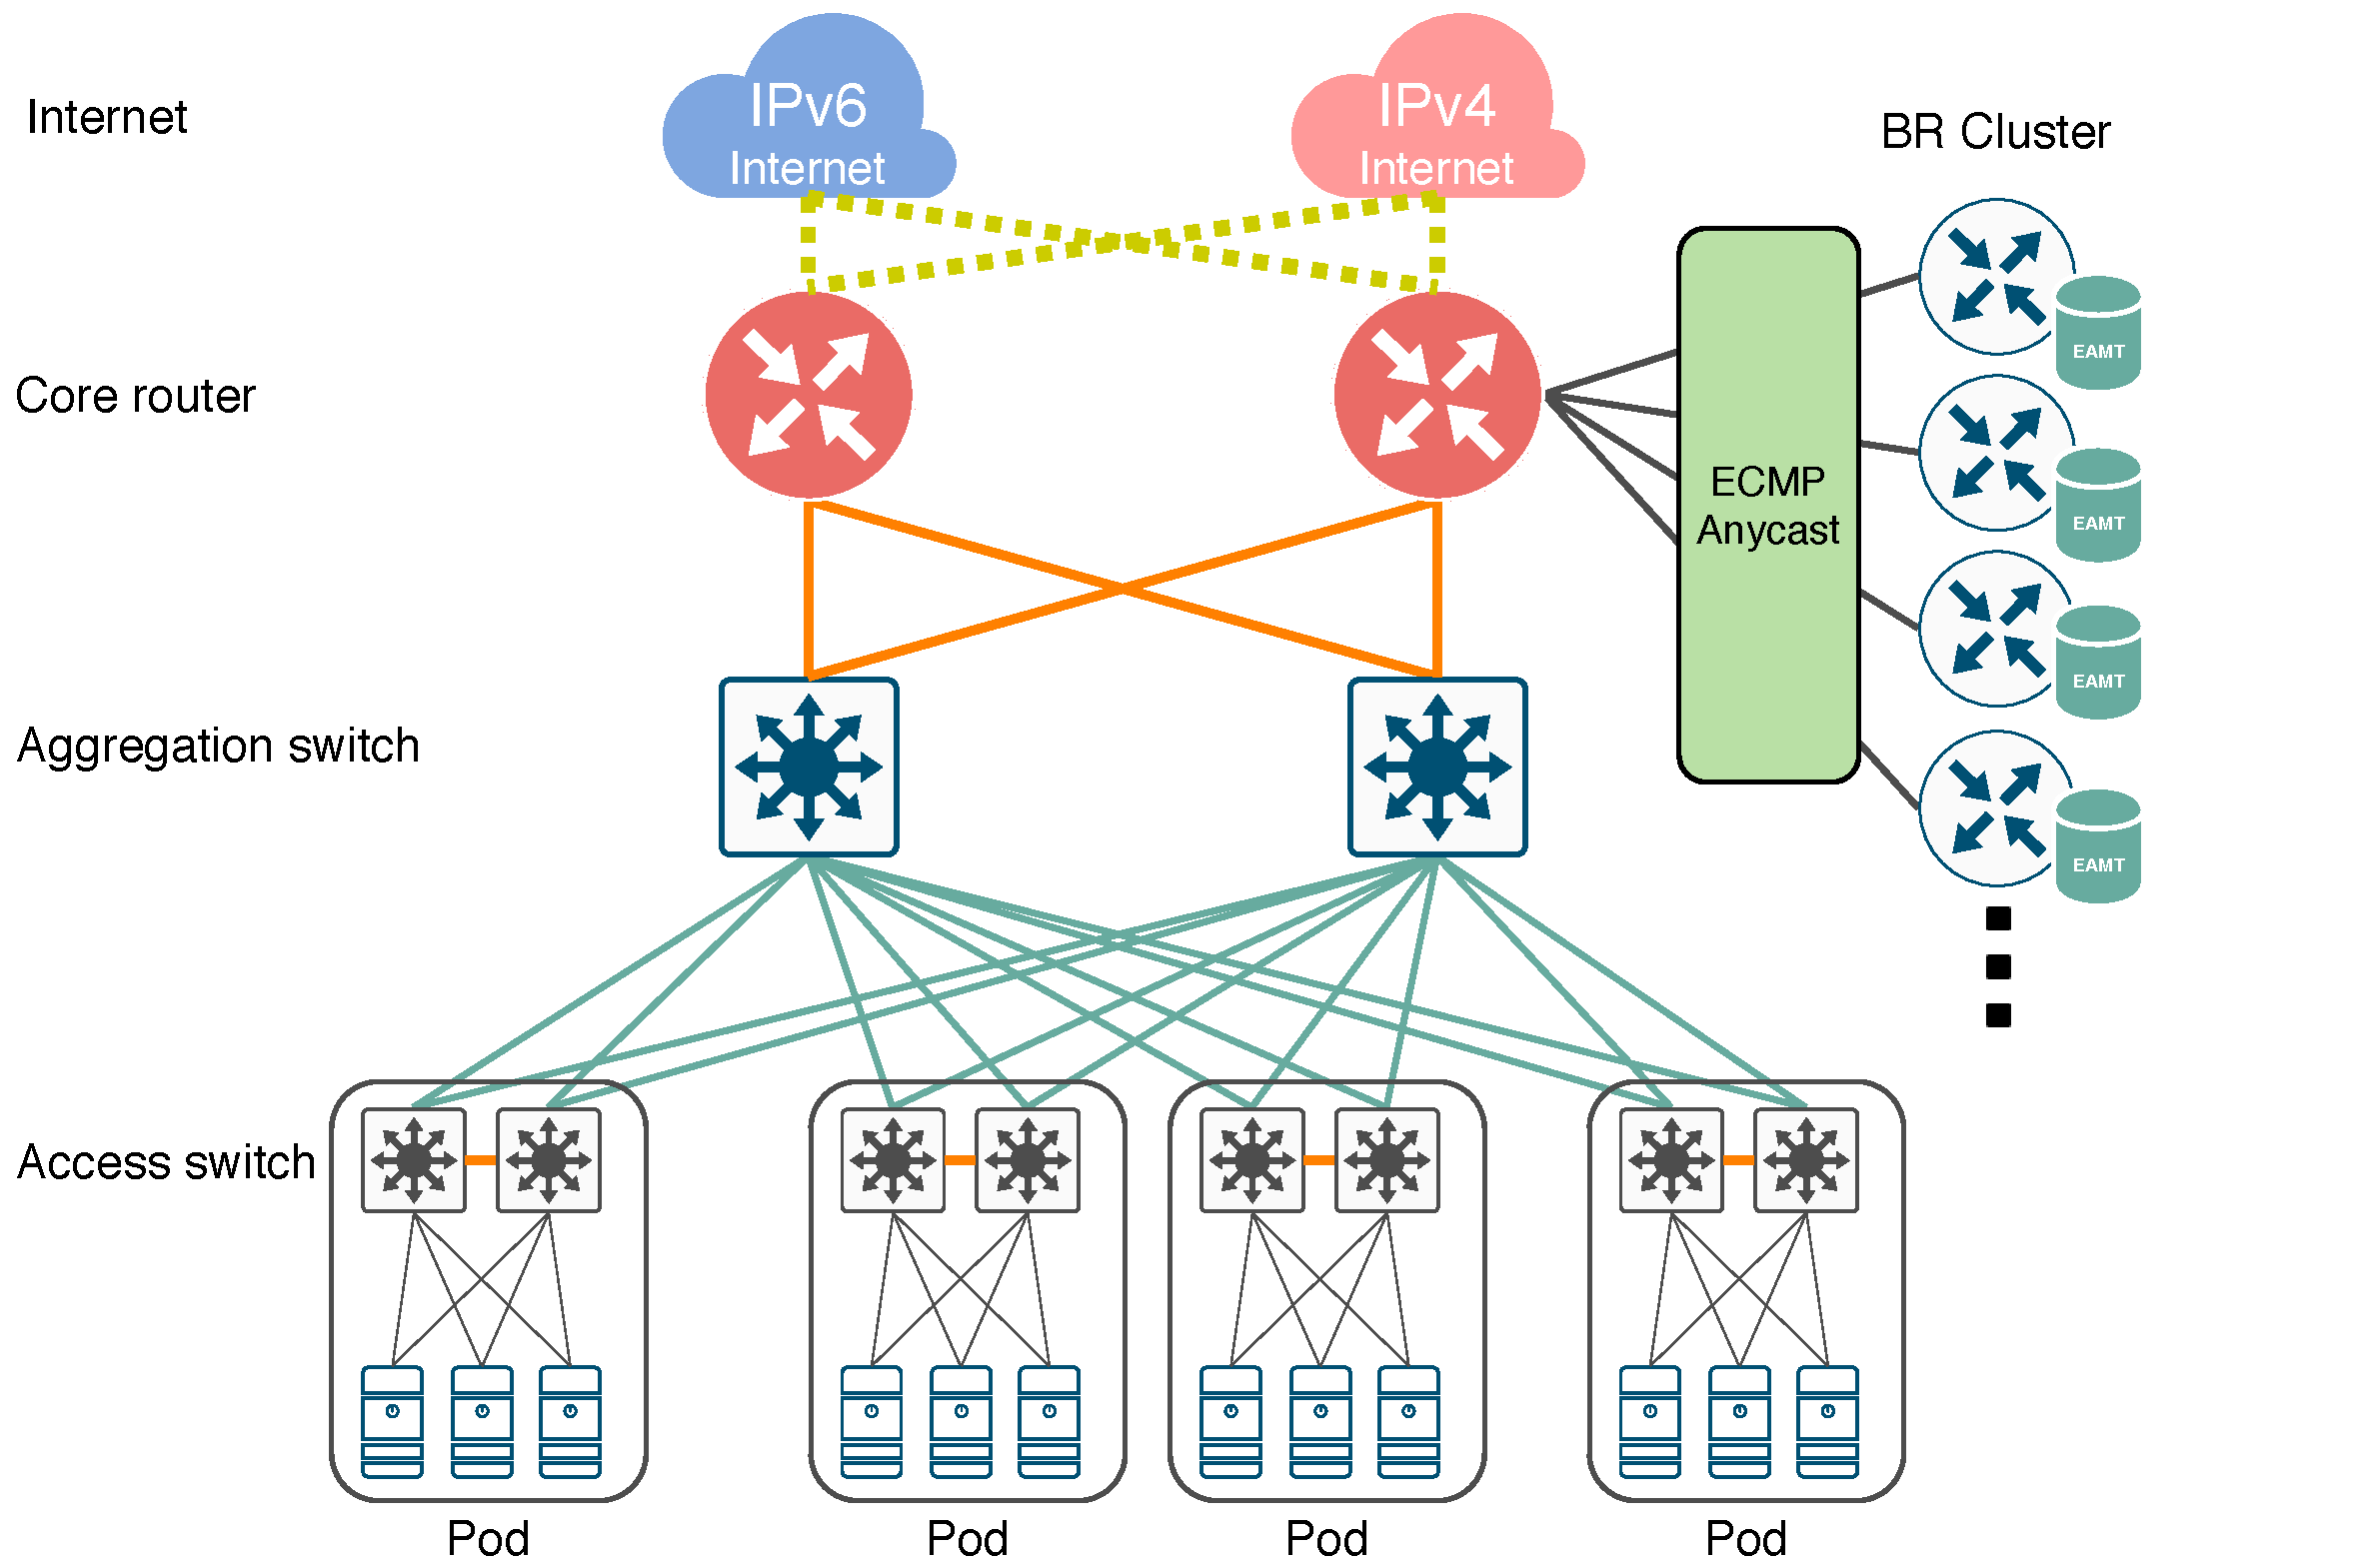
\includegraphics[width=12cm,pagebox=cropbox,clip]{img/siit-dc_scale.pdf}
  \end{center}
  \caption{BRを水平スケールすることが出来るSIIT-DCネットワーク}
  \label{fig:siit-dc_network_scale}
\end{figure}

BRはIDCのIPv6ネットワークIPv4インターネットに接続するためのネットワーク疎通性を用意することでサービスを行う.そのため,ECMP及びエニーキャスト\cite{RFC4786}を利用して,BRの数を追加するのみによって,IPv4サービスの提供容量を増加させる事ができる.

図\ref{fig:siit-dc_network_scale}にスケーラビリティを意識したBR配置を行ったネットワークの例を示す.IPv4クライアントからのアクセスは一度いずれかのBRにフォワーディングされた後,IPv6プロトコルに変換された上で再度コアルーターを介してIDCネットワークに到達する.



\subsection{基本的なパケットの流れ}
\label{issue:siit-dc:packet_flow}

\begin{figure}[h]
    \begin{center}
      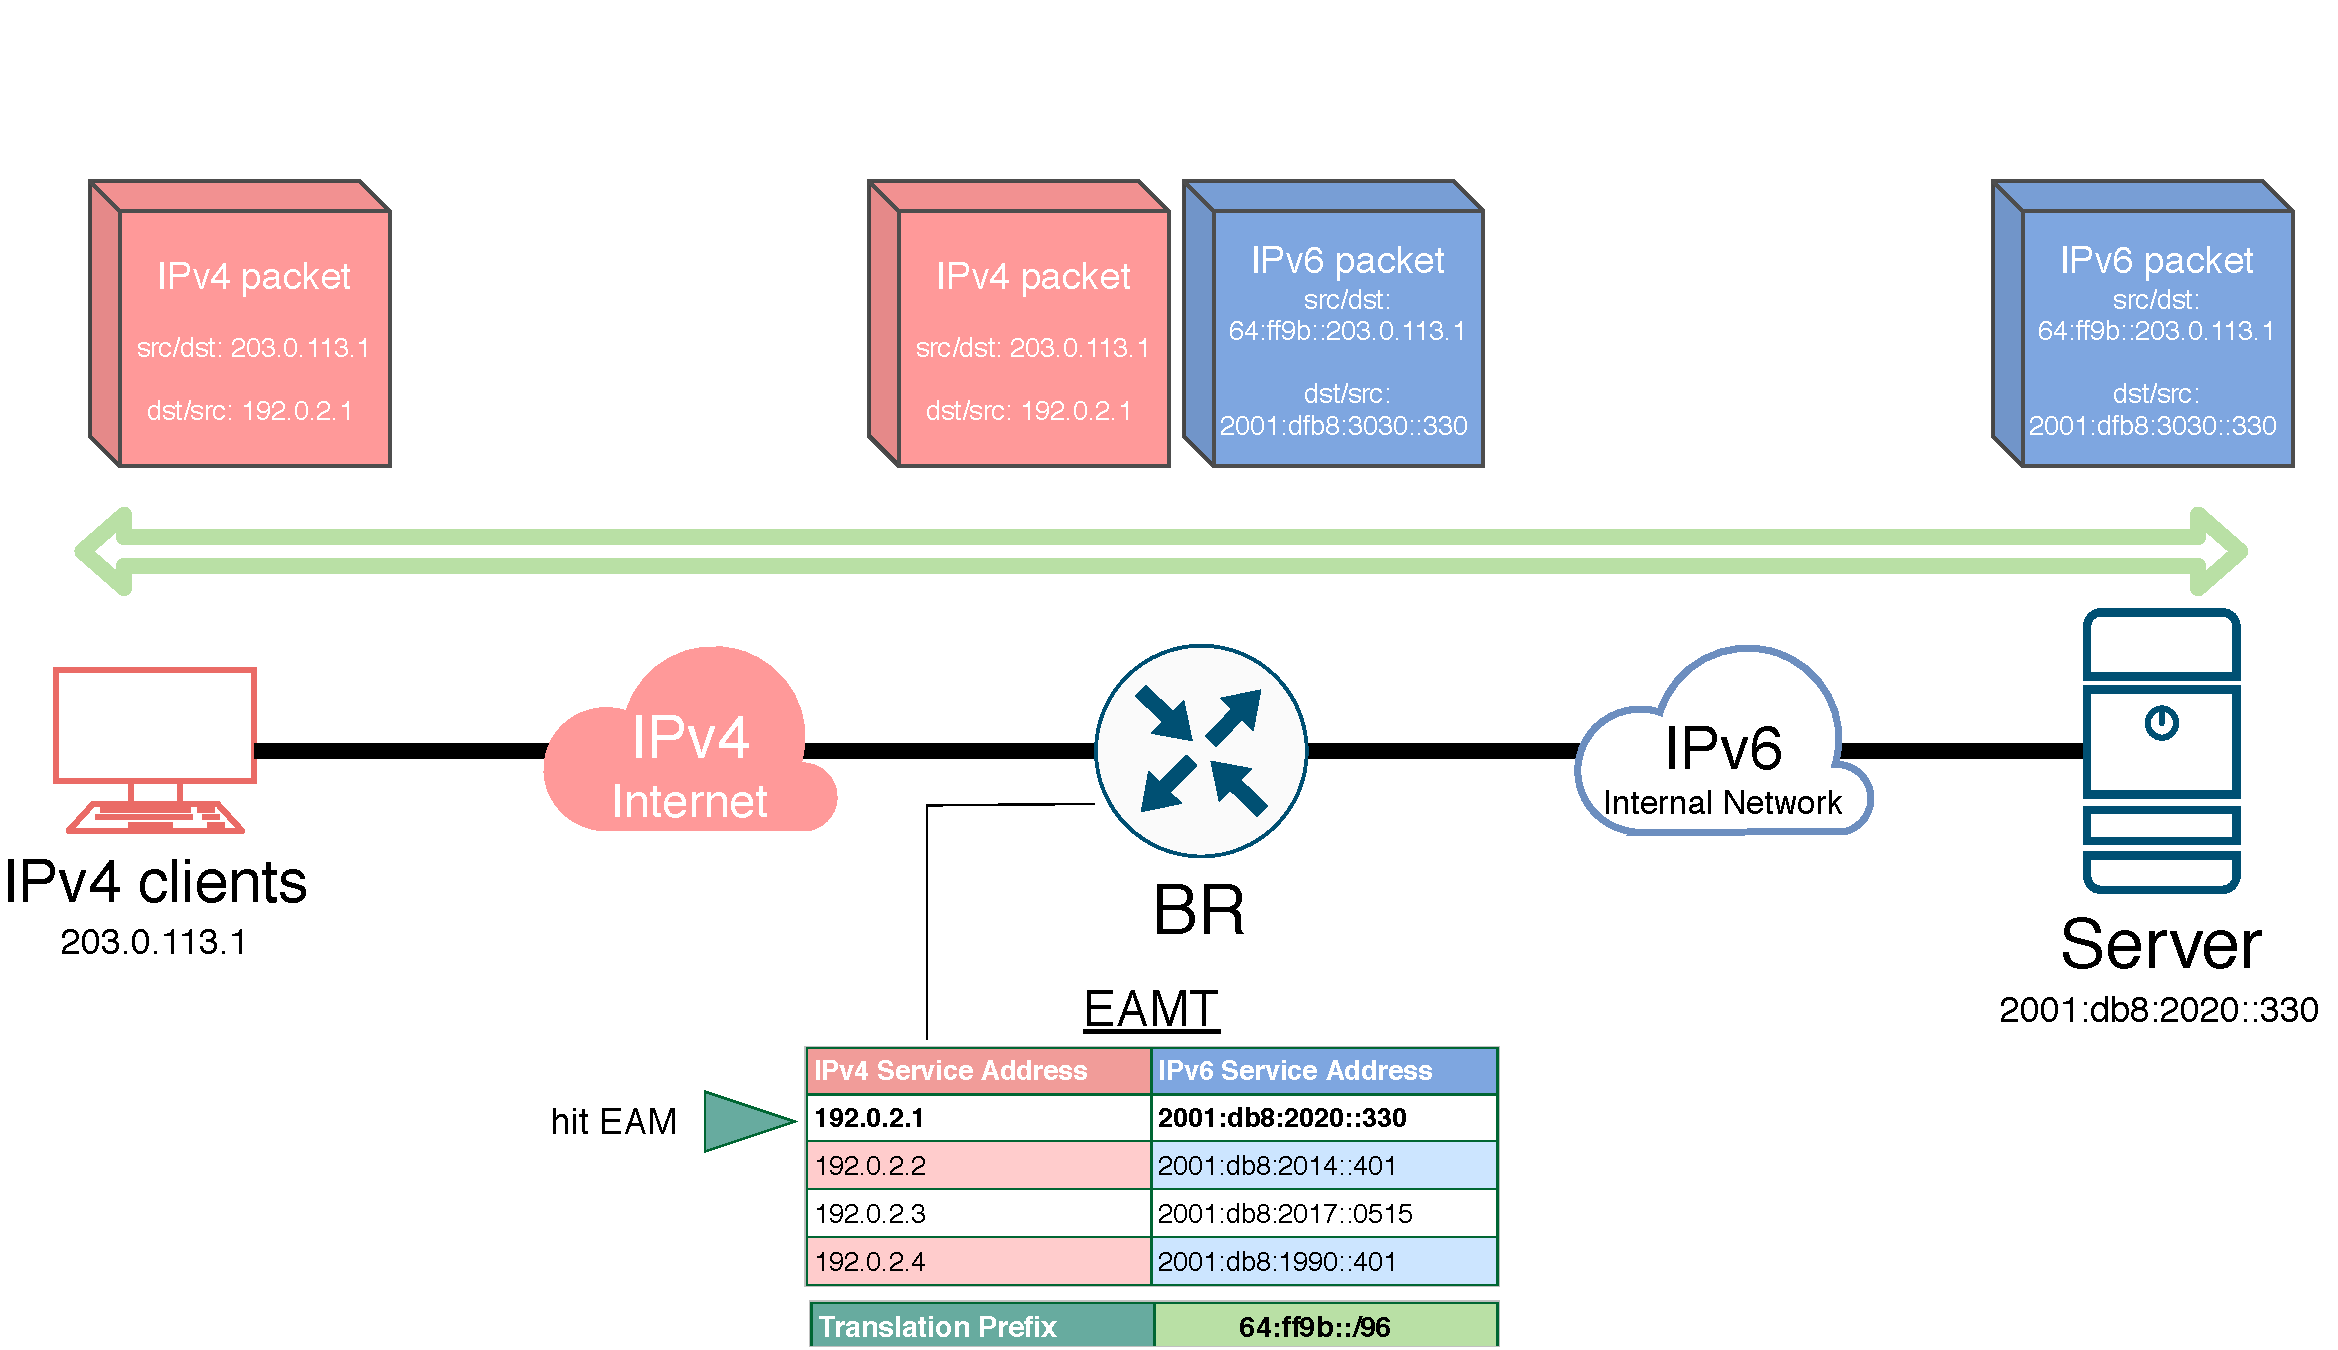
\includegraphics[width=14cm,pagebox=cropbox,clip]{img/siit-dc_packet.pdf}
    \end{center}
    \caption{SIIT-DC パケットの流れ}
    \label{fig:siit-dc_packet}
\end{figure}

SIIT-DCにおける基本的なIPv4クライアントからのトラフィックの流れは以下の様になる.一連のパケットの送信元・送信先のアドレスの遷移を図\ref{fig:siit-dc_packet}に示す.

IPv4クライアントのIPv4サービスアドレス宛のパケットはIPv4インターネットに接続するBRに到達後,当該BRが有するEAMTに従ってIPv6サービスアドレス宛のIPv6パケットに変換される.このパケットの送信元アドレスは変換プレフィックスに埋め込まれたIPv6アドレスとして表現される.IDC内のIPv6ネットワークを介してIPv6サーバーに到達した後,IPv6サーバーは送信元アドレスへの応答パケットを送信する.第\ref{issue:siit-dc:translation-prefix}項で述べたように,変換プレフィックス宛のパケットはIPv6ネットワークを経由してBRにルーティングされる.IPv6サーバーからの応答を受け取ったBRはEAMTを参照し,送信元アドレス(IPv6サービスアドレス)をIPv4サービスアドレスに書き換え,送信先アドレス(IPv4クライアントのIPv4アドレス)から変換プレフィックスを除去書き換えたのち,IPv4インターネットを介してIPv4クライアントに返送される.




\section{SIIT-DCの課題}
\label{issue:siit-dc_problems}
本節ではSIIT-DCの現状の課題及びそれに起因して起こる事象に関して述べる.

\subsection{一貫したEAMTの必要性}
\label{issue:siit-dc_problems:consistent}

\begin{figure}[h]
    \begin{center}
      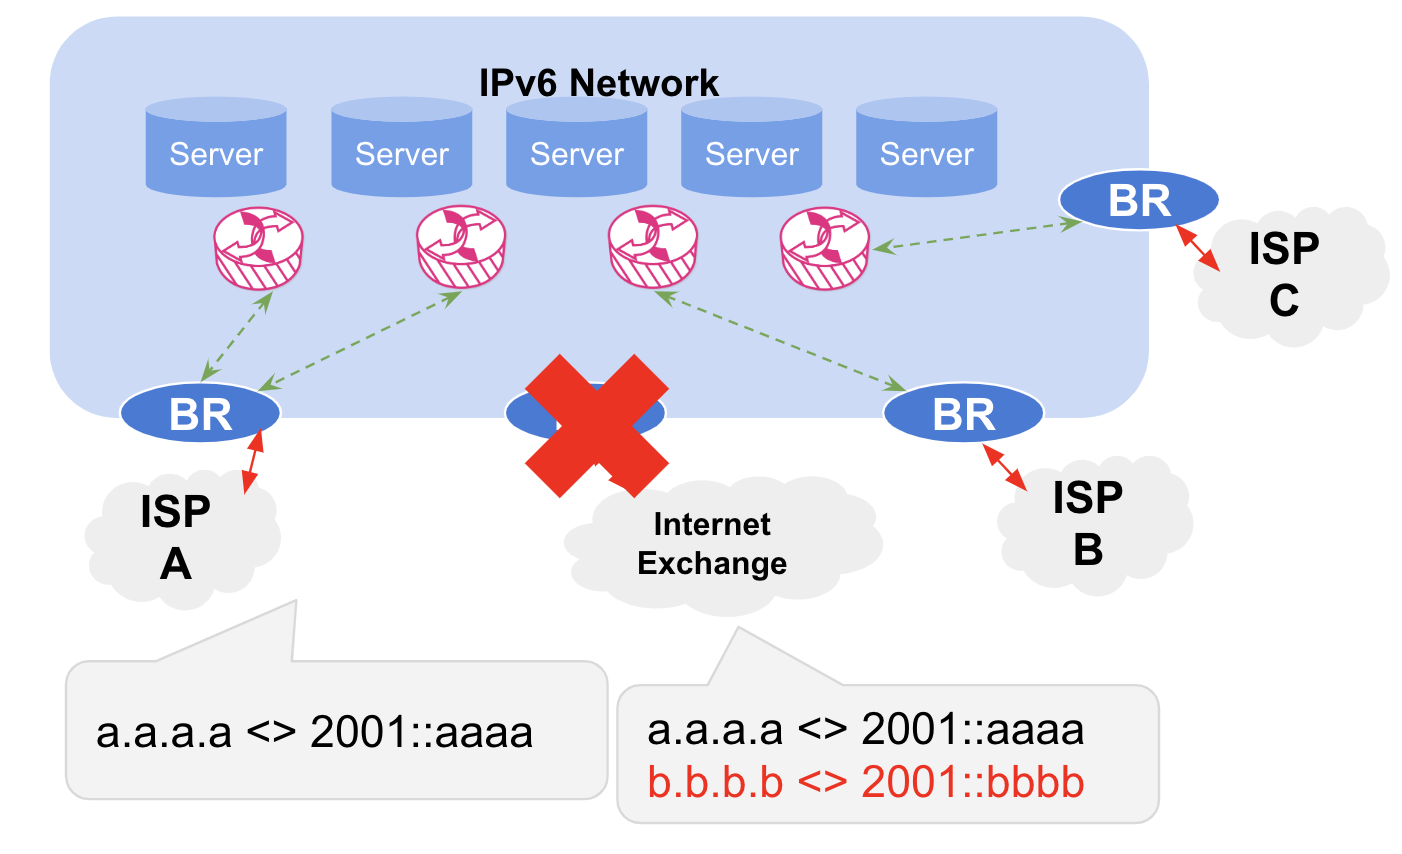
\includegraphics[width=10cm,pagebox=cropbox,clip]{img/siit-dc_can-not-failover.png}
    \end{center}
    \caption{BRに障害が発生した場合に適切にフェイルオーバーが出来ないケース}
    \label{fig:siit-dc_can-not-failover}
\end{figure}

第\ref{issue:siit-dc:terms}で述べたように,SIIT-DCでは対外接続点ごとにBRを配置するネットワークデザインを採用することで,IPv6シングルスタックネットワークに最小限のIPv4ネットワークを追加するのみによりIPv4サービスの提供を可能にしている.また第\ref{issue:siit-dc:network}項や第\ref{issue:siit-dc-merit:scalability}項で触れたように,複数のBRで共通した変換プレフィックスをエニーキャストでIDCネットワーク内に広告する運用を行うことにより,BR及び対外接続点の障害時に他のBRを用いてIPv4サービスの提供を継続することが出来る.この機構を有効に作用させるためには,SIIT-DCネットワーク内の全てのBRで一貫したEAMTの保持が求められる.

しかしながら現状のSIIT-DC及びEAMTの仕様\cite{RFC7755,RFC7756,RFC7757}では,BRは他のBRとの間でEAMTを共有するためのメッセージング機構を有さない,これはBR間でEAMTの不一致が発生した場合に,差異となったEAMに該当するIPv4サービス宛のトラフィックの別のBRへの迂回が出来なくなるケースが発生することを意味する.


\subsection{変更追従性の欠如}
\label{issue:siit-dc_problems:follow}

\begin{figure}[h]
    \begin{center}
      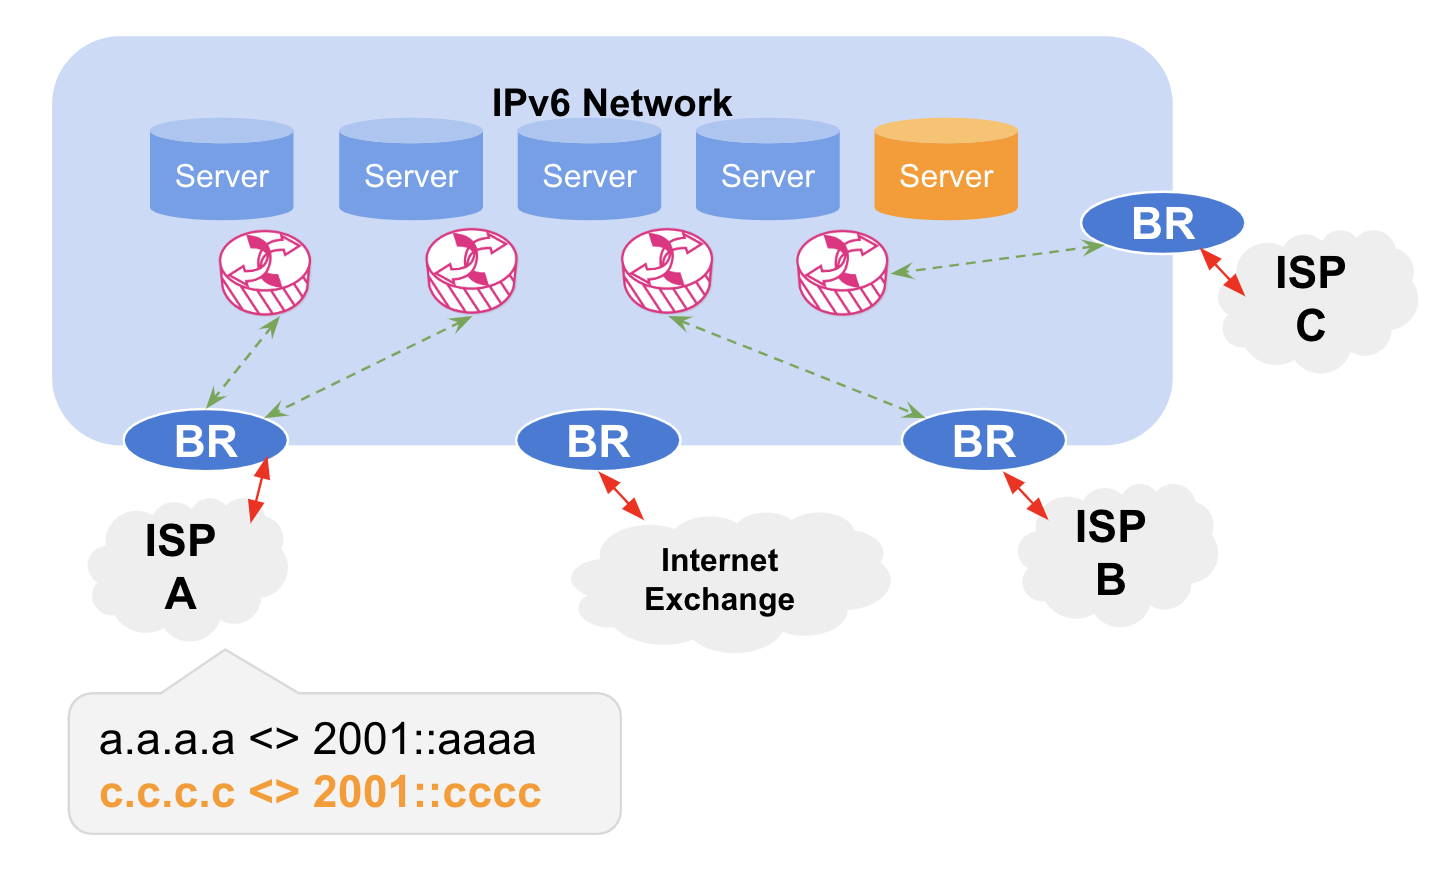
\includegraphics[width=10cm,pagebox=cropbox,clip]{img/siit-dc_add-server.png}
    \end{center}
    \caption{サーバーを追加した際,全てのBRへの設定追加が必要になる.}
    \label{fig:siit-dc_add-server}
\end{figure}

プライベートクラウド環境が一般的に利用されるIDCネットワークでは,日々多くのサーバーやアプリケーションが追加・廃止・変更される.
一方で第\ref{issue:siit-dc_problems:consistent}で触れたように,SIIT-DCでIPv4提供サービスを冗長に運用するためには,IPv4提供サービスに該当するEAMがBRのEAMTに保持されることを要求している.IPv4提供サービスの構成に変更があった場合,全てのBRのEAMTに対してEAMの更新を行わなくてはならない.

しかしながら現状SIIT-DC及びEAMTの仕様\cite{RFC7755,RFC7756,RFC7757}において,IPv4サービスを行うサーバーの存在や状態によってダイナミックにEAMTを更新する機構は存在しない.そのため,IDCネットワークにおけるIGPなどによってIPv6サービスへの到達性が検証されていたとしても,IPv4サービスの場合はリアルタイムな構成変更に追従することが出来ない.



%%% Local Variables:
%%% mode: japanese-latex
%%% TeX-master: "./thesis"
%%% End:
